%
\chapter{Implementation}\label{cha:Implementation}
%
In this chapter, the implementation part of this master's thesis will be described. The test track, which was built before by another student; the hardware part of the model automobile, which was used in this master's thesis; and finally, the software part which was programmed for detecting the lanes will all be  explained in detail.

In the Software section in \ref{sec:Software}, all methods programmed and utilized during this master's thesis will be described. In order to better demonstrate the process, pictures of each step, as well as block diagrams of each method, will be shown.

%
\section{Test Track}\label{sec:Test Track}

As previously mentioned, the medium-term goal of this master thesis is attending the Carolo-Cup at Braunschweig University, so the test track was prepared according to the Carolo-Cup criteria by Nicolas Acero Sepulveda, who also did his bachelor's thesis with this model automobile. For this test track, two black PVC floor carpets were used and on these floor carpets, the lanes of the track were made by using white electrical tape. The straight part of the track was made on one of these PVC floor carpets and the curved part of track was made on the second PVC floor carpet. The straight part of the track is approximately 2 meters long and the curve radius of the curved part of test track is approximately 1 meter. This curve is the tightest curve at Carolo-Cup, so with this, the test track can be tested in the worst case scenario. In the Carolo-Cup competition, the track is much larger; however, for the purposes of this master thesis, a larger test track in not needed. In Figure \ref{fig:Test_Track}, the test track used in the testing of this master's thesis is shown.


\begin{figure}[H]
	\centering
		\includegraphics[width=1\textwidth]{./Bilder/Test_Track.jpg}
	\caption{Test Track}
	\label{fig:Test_Track}
\end{figure}



%
\section{Hardware}\label{sec:Hardware}

While working on a software project, though it is of course important to write an efficient software, it is also important to choose the right hardware. In this project, the model automobile was already prepared for a project course at the Technical University of Darmstadt. However, for this project, it was necessary to use another camera for lane detection, as the original was not sufficient for this purpose. In this chapter, the hardware component of this project and the changes made to the model automobile will be described.


%
\subsection{Model Auto}\label{sec:Model Auto}


During the course of this master's thesis, a model automobile which was prepared for the Projectseminar Echtzeitsysteme at Technical University of Darmstadt was used. The chassis, steering mechanism, power train, and engine control were derived from the model-building of a Japanese company, Tamiya. The maximum velocity of the model automobile is approximately \emph{\color{green}1 m/s} and the minimum steering radius is around 90 cm. 

\begin{figure}[H]
	\centering
	\hspace*{0cm}   
	\includegraphics[width=150mm,scale=1]{./Bilder/Model Auto.jpg}
	\caption{Model Auto}
\end{figure}

%
\subsection{Microcontroller and Main Board}\label{sec:Microcontroller and Main Board}


In this model automobile, there is a microcontroller and a main board. The microcontroller is used for controlling steering 
and receiving the measurements from ultrasonic sensors and hall effect sensors. The 16-bit microcontroller is from 
MB96300 series from Fujitsu company.

The main board on the model car is from PD10BI-MT ThinMini-ITX series from the MiTAC company. This main board communicates 
with the microcontroller over an UART interface through USB connection. On this main board, according to the website of the MiTAC company\cite{PD10BIMT}, there is an Intel Celeron J1900 Quad core processor with integrated graphics. Furthermore, there is an 8 GB DDR3-1600 RAM and 1Gbit/s Ethernet, VGA, HDMI, USB 2.0/3.0, SATA ports and an Intel Dual Band Wireless AC 7260 Network adapter, which is connected to two external WLAN antennas. A 60 GB Kingston SSD-Harddisk is connected over an integrated PCI-Express Port. A 3200 mAh Li-Fe battery is used as a power supply.
%

\subsection{Camera}\label{sec:Camera}


The camera is one of the main components of lane detection and accordingly, autonomous driving. For this thesis, I had 
to research the most suitable camera because all cameras have different properties.

At the beginning of the Projectseminar Echtzeitsysteme, the Logitech C270 HD Webcam was being used. The resolution of 
the camera is 1280x960 pixels and the Frame per Second (FPS) value is 30 Hertz (Hz) at a 640x480 pixel resolution. 
The field of View (FOV) is just 60 degrees. The problem with this camera is that if there is a curve, the camera 
cannot see all of the lanes, and thus is not very suitable for lane detection. When I started my master's thesis, there 
was a Kinect v2 camera on the model car.  The Kinect v2 camera was developed by Microsoft and released in 2013. This 
camera has a depth sensor with a resolution of 512x424 pixels and its FOV is 70x60 degrees. The FPS value is 30 Hz at 
a 512x424 pixel resolution. This camera also has a color camera with resolution of 1920x1080 pixels and a FOV of 
84.1x53.8 degrees. The FPS value is 30 Hz at a 1920x1080 pixel resolution. This camera had two main disadvantages for 
this master's thesis. The first disadvantage is the FOV value of camera. This value is better than the value of Logitech 
C270 camera but it is still not enough for curve lane detection. The second main disadvantage is the location of the 
color camera. The color camera of this camera is not in the middle of camera, but on the right. This is a 
disadvantage for us because when there are curves going left as opposed to right, the camera is unable to see the 
left and even perhaps the middle lane of the track. Thus, this is problematic for lane detection.

Due to these reasons, it was necessary to select a camera which has a sufficiently high FOV value. After doing research, I decided 
that the Genius Widecam F100 camera is the best choice for this master's thesis because this camera has a FOV value of 
120 degrees and it can also be used with the Linux Operating System. The resolution of this camera is 1920x1080 pixels 
and the FOV value is 120 degrees. The FPS is 30 Hz at a 1920x1080 pixel resolution. With this camera, it is possible 
to detect most if not all lanes, including when there are curves. 


\begin{figure}[H]
 \centering
  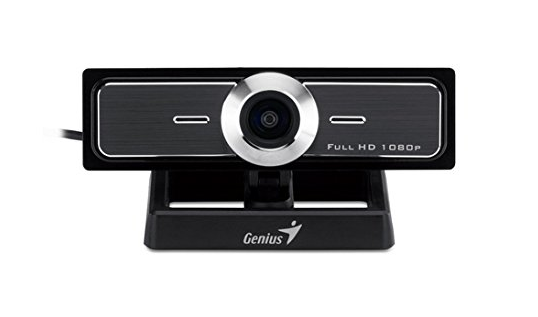
\includegraphics[width=1\textwidth]{./Bilder/Genius_F100_camera.png}	
   \caption{Genius 120-degree Ultra Wide Angle Full HD Conference Webcam(WideCam F100) }
  \label{fig:Genius-Camera}
\end{figure}






\section{Response Time of the System}\label{sec:Response Time of the System}

Before the lane detection project was started, it was necessary to conduct an experiment with the system. The aim of this experiment was to measure the response time of the entire system. In order to measure it, the camera had to detect something and then the software had to set an I/O pin on the main board. The amount of time this process took was in fact the response time being searched for.

For this experiment, a camera, a function generator, an LED, and an oscilloscope were needed. A circuit with a power supply and an LED were designed. The LED was placed in a small box with a camera, and one probe of an oscilloscope was connected to the LED while its other probe was connected to an I/O Pin on the mainboard, which could be set with software.

Before the results were measured, the frequency of the camera was set to 10 Frames per Second(FPS) and the power supply was set to 3.28 Hz square wave. This means that the LED is supposed to blink approximately every 305 ms.

After the supply was turned on, the LED started to blink. For this experiment, a small firmware able to detect the color red was written in order to detect when the red LED lit up.

The LED and a camera were placed together in a box and the box was closed, and so the inside of the box was totally dark. When the red LED lit up, the camera detected it and the firmware set an I/O pin on the main board. For this experiment, two different cameras (Logitech Webcam C270 model and Logitech Webcam C905 model) were used and the results were very similar.


\begin{figure}[H]
 \centering
  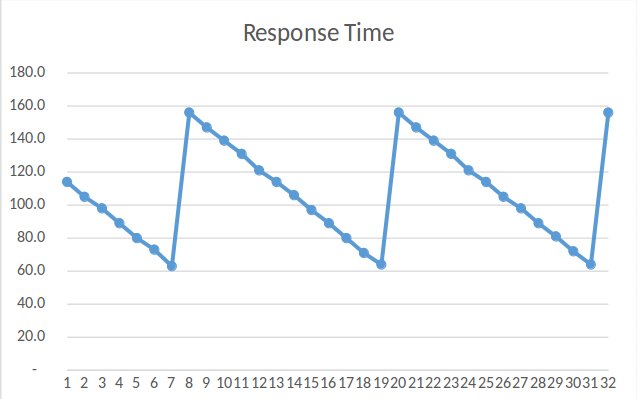
\includegraphics[width=0.8\textwidth]{./Bilder/Response_Time2.png}		 \caption{Response Time of the System} 
  \label{fig:Response_Time_of_the_System}
\end{figure}


As in Figure \ref{sec:Response Time of the System} seen, the maximum response time of the system was 156 ms, the minimum response time of the system was 63 ms, and the average time was 106.6 ms.

This Figure shows that the frames are steadily sent by the camera. In addition, if the LED lights up and is immediatly followed by new frame, then the light is detected. If the LED goes dim and is followed by a new frame, then the response time of the system is minimum, which is measured at 63 ms. On the other hand, if the frame comes and then immediately the LED changes its status (on/off), the new status of the LED is not detected until the new frame is received. The FPS value of the camera is ten, which means that the system must wait nearly 100 ms for the new frame and after that, the response time of the system must taken into account, so the maximum response time of this total system is around 156 ms. This means that the FPS value of the camera is important for response time of the entire system. Because it is desirable to increase the FPS value of the camera, decreasing the computing times of lane detection methods is also desirable, as this would allow for an increase in the FPS value.




%
\section{Software}\label{sec:Software}


In this chapter, the software algorithms defined in this master's thesis will be focused on. With the aid of program flow charts and explanations of all their steps, the algorithms will themselves be explained in detail. In order to find the best solution, five different source code versions were generated. For all these source codes, the computing times were calculated and compared in terms of which solution can detect the lanes better. In the following pages, there are detailed explanations of the methods utilized. The development environment and the software utilized in this master's thesis will be also described.

%
\subsection{Development Environment and Related Software}
\label{sec:Development Environment and Related Software}

As also mentioned at subsection \ref{sec:Microcontroller and Main Board}, in this project the previously introduced main board was utilized. One of the compact and fast versions of the Linux 16.04 operating system, \textit{Lubuntu} was installed in this main board.

The version \textit{Kinetic} of ROS was used for implementation of this master's thesis. ROS is the abbreviation of \textbf{R}obotic \textbf{O}perating \textbf{S}ystem, which is a flexible framework for writing robot software (i.e. collection of tools and libraries for robot software development). On the ROS wiki page\cite{ROS}, ROS is defined as an open-source, meta-operating system for your robot. It provides the services you would expect from an operating system, including hardware abstraction, low-level device control, implementation of commonly-used functionality, message-passing between processes, and package management. It also provides tools and libraries for obtaining, building, writing, and running code across multiple computers.

For using prepaid image processing functions, an open-source computer vision and machine learning software library called OpenCV was used. According to the OpenCV website\cite{OpenCV_About}, there are more than 2500 optimized algorithms in the OpenCV library and OpenCV has a user community of more than 47 thousand people.

ROS can be programmed with Python, C++ or Lisp programming languages and OpenCV can be programmed with Python or C++ programming languages. In this master's thesis, C++ was used.

Because the monitor cannot always be connected to a PC via a cable for practical reasons, in order to see if the algorithm can detect the lanes, the on-board PC must be connected to a PC remotely. For that, there is a software used which can connect two different computers which are run by the Linux operating system. As the first step, a wireless network must be created in one of these computers and the other computer must be connected to this wireless network. Then the IP address of the model car must be determined or a static IP address must be given to the model automobile. As the last step, 'Remmina Remote Desktop Client' must be used in the PC and the IP address of the model automobile (Server) must be given. After that, the model automobile and the PC are connected to each other. In this software, the quality of screen sharing and the speed can be adjusted.  

%
\subsection{Preprocessing}\label{sec:Preprocessing}

There are many different possibilities for lane detection algorithms. Of course, each has its own advantages and disadvantages. In this master's thesis, some methods were defined, and in this chapter, these methods will be explained in detail.

In all of these methods, some processes are common, and this is called the preprocessing part. In Figure \ref{fig:Block_Diagram_of_the_Preprocessing_Part}, the steps of the preprocessing part are shown.

At the beginning, the frames are obtained from the camera via ROS-Topic. ROS uses different image formats than OpenCV, which uses the image format Matrix(Mat). The frame obtained via ROS-Topic must be converted from the ROS image data type to a Mat object. In order to convert the frame, a ROS-Package \textit{cvbridge}\cite{cv_bridge} was used. cvbridge converts the ROS image format to a Mat Object, which is the OpenCV Image Format. 

Mat is a class which has two parts. The parts are a matrix header and a pointer to the matrix containing the pixel values. The matrix header contains information like the size of matrix, storing method, etc. It always has a fixed size but the size of matrix is variable from image to image.

There are many methods which can store the pixel values to the Mat object. In this case, the color space and the data type utilized can be chosen. For gray images, it is easy to choose the color space because there are just two colors : black and white. By changing the density of colors(black and white), it is possible to create many shades of gray. There are more methods for color images. Color images generally have three or four channels. These three channels are used for RGB color values. The RGB colors are based on the colors red, green, and blue, which can all be detected by the human eye. For the transparency of a color, a fourth channel called alpha(A) can be used.

There are also another color formats, which have some advantages\cite{OpenCV_Mat}. 

\begin{itemize}

\item The RGB format is quite similar to the human eye, but the OpenCV display system uses the BGR format, which uses another order of colors.

\item The HSV and the HLS formats are more natural ways to display colors. They decompose colors into their hue, saturation, and value/luminance components. Another advantage of the HSV and the HLS formats is that they are less sensitive to the light conditions of the input image.

\item In JPEG image formats the YCrCb format is used.

\item If the distance of a given color to another color is to be measured, CIE L*a*b* format is more suitable than others.

\end{itemize}




\begin{figure}[H]
 \centering
  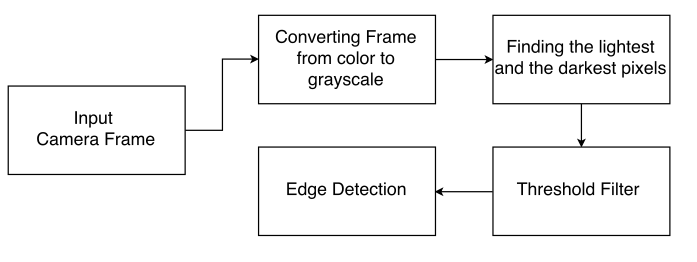
\includegraphics[width=1\textwidth]{./Bilder/Presprocessing_Figure.png}	
  \caption{Block Diagram of the Preprocessing Part}
  \label{fig:Block_Diagram_of_the_Preprocessing_Part}
\end{figure}





After the frame from Camera via ROS-Topic is received, the color frame has to be converted to a grayscale frame. For detection lanes, Hough Transformation is used and for Hough Transformation, the grayscale format of the input image is needed. Converting a frame from BGR format to grayscale format has some advantages, the main advantage being the processing time. Normally color frame matrix content has three or four channels, but grayscale frame matrix content has just one channel, so grayscale frame matrix size is much smaller compared to color frame matrix size. Because of this, the image processing time is much less for the grayscale format compared to BGR format. In order to convert the BGR formatted frame to a grayscale formatted frame, the \textit{cvtColor} function from OpenCV is used.

For stable lane detection, the light conditions must be considered. Because of this, after converting the frame with BGR format to grayscale format, the lightest and darkest pixels have to be searched for. In order to find the lightest and the darkest pixels, the following function in OpenCV was used. This function will be explained in detail.\cite{addWeighted}


\begin{center}

\texttt{void minMaxLoc(InputArray src, double* minVal, double* maxVal=0, Point* minLoc=0, Point* maxLoc=0, InputArray mask=noArray())}

\end{center}

\begin{itemize}

\item \textbf{src : }Input single channel array.

\item \textbf{minVal : }Pointer to the returned minimum value.

\item \textbf{maxVal : }Pointer to the returned maximum value.

\item \textbf{minLoc : }Pointer to the returned minimum location.

\item \textbf{maxLoc : }Pointer to the returned maximum location.

\item \textbf{mask : }Optional mask used to select a sub-array.

\end{itemize}


After finding the lightest and darkest pixels, it is possible to estimate the lighting conditions. These values are then used in the next step. After this processing, a filter is applied to all frames, transforming images into binary images by transforming each pixel according to whether it is inside or outside a specified range. The user chooses a threshold value to process. If a pixel is greater than this value, it is assigned an 'inside' value; otherwise, it is assigned an 'outside' value. Depending on the lightest and darkest pixel values, the threshold value changes. Through this dynamic parameter, the lanes are more able to be more clearly detected and noise can be cancelled more successfully. For this thresholding operation, the following function in OpenCV was used. This function will be explained in detail\cite{threshold}.


\begin{center}

\texttt{double threshold(InputArray src, OutputArray dst, double thresh, double maxval, int type)}

\end{center}

\begin{itemize}

\item \textbf{src : }Input single channel array, which is 8-bit or 32-bit floating point.

\item \textbf{dst: }Output array which has the same size and type as src. 

\item \textbf{thresh : }Threshold value.

\item \textbf{maxval : }Maximum value to use with the THRESH\_BINARY and THRESH\_BINARY\_INV thresholding types.

\item \textbf{type : }Thresholding type, which can be THRESH\_BINARY, THRESH\_BINARY\_INV, THRESH\_TRUNC, THRESH\_TOZERO and THRESH\_TOZERO\_INV.

\end{itemize}




After the threshold filter, an edge detection filter must be applied. In this master's thesis, the Sobel-Operator is used. This is explained in Chapter 2 in detail.
 
This preprocessing part is common for all cases but after this process, the cases diverge. 
 
%
\subsection{Method 1 : Hough Transformation + Rectangle Method + Curve Fitting + IPM}\label{sec:Case 1}

The algorithms and their orders which was used in this method, will be explained step by step. At Figure \ref{fig:Case1_BlockDiagram}, the block diagram of Method 1 is shown.



\begin{figure}[H]
 \centering
  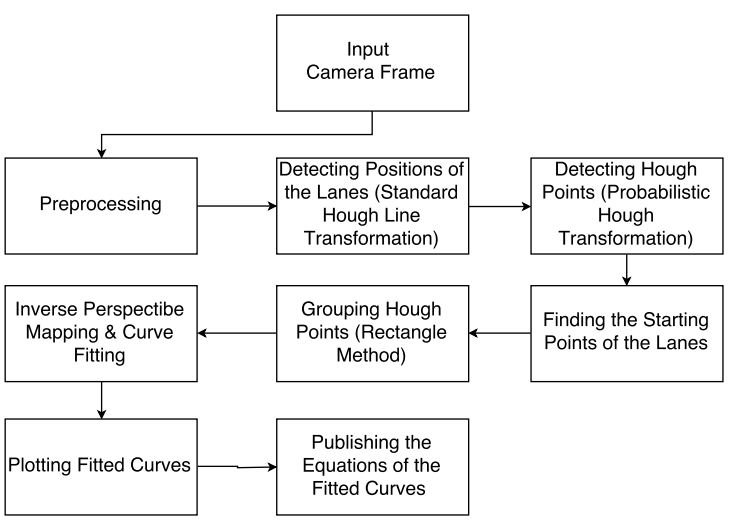
\includegraphics[width=1\textwidth]{./Bilder/Case1_BlockDiagram.png}		 \caption{Block Diagram of Method 1}
  \label{fig:Case1_BlockDiagram}
\end{figure}



\textbf{Step 1 : }As with all methods, the first step is the preprocessing phase. When the preprocessing phase is over, it must be determined which pixel columns the lanes lie between. 

\textbf{Step 2 : }Secondly, the positions of the lanes should be found. In order to find the positions of the lanes, the Standard Hough Line Transformation is used. But the Standard Hough Line Transformation should not utilize the entire frame; rather, the frame is cropped. There is an advantage to cropping the frame, which will be explained in detail.


In this project, the Standard Hough Line Transformation is used differently than usual. Normally, the Standard Hough Line Transformation detects the straight lines but here, it checks if there are two edges in the same pixel column of the frame. In other words, if there is a lane, there are two edges of the lane in the frame so if there is a lane, there are also Hough Transformation lines. For the Standard Hough Line Transformation, the function of OpenCV is used. As previously explained in Section \ref{sec:Standard Hough Line Transformation}, in order to use this function in OpenCV, some parameters must be set. One of these parameters was the 'threshold', which decides the minimum number of the points to detect a line. In a lane, there are two edges, so the Standard Hough lines must be drawn if two points in the same vertical are detected. These two points are only searched for vertically, so another parameter in the Standard Hough Line Transformation function from OpenCV is used for the angle, which has to check the points in that angle. Because only vertical edges are checked, this angle value, named '$\theta$', is set to 'CV$\_$PI(180 degree)'.


 
The frames obtained from the camera are at a resolution of 640x480 pixels, which is the default value. The resolution of the camera can be increased and decreased by adjusting its settings.
The original height of the frame was 640 pixels in this method, but as previously mentioned, the frame was cropped. As seen in Figure \ref{fig:Case1_withoutCropped}, the camera detects the edges that do not belong to the track. When the frame is not cropped, the detection of irrelevant edges would result in the undesired production of Standard Hough Transformation lines (shown in red).  Thus, the Hough Transformation is only used for the lower 230 pixels, if more than 230 pixels are used for generating the Standard Hough Transformation lines. 

As seen in  Figure \ref{fig:Case1_withCropped},  the red lines are shown only in the last 230 pixels of frame height and do not cover the irrelevant parts of the frame. If there is a lane, the red lines are very close to each other, but if there is no lane, there is a distance of at least 50 pixels between the red lines. In Figure \ref{fig:Case1_withCropped}, there are two different groups of red lines. In each group, there is a lane. Thanks to the Standard Hough Line Transformation, it is known which lanes are between which pixel columns. The group of Standard Hough Transformation lines on the right indicates the right lane and the group of Standard Hough Transformation lines on the left indicates the middle lane. 

\begin{figure}[H]
  \centering
  \subfloat[Standard Hough Transformation without Cropping Image]{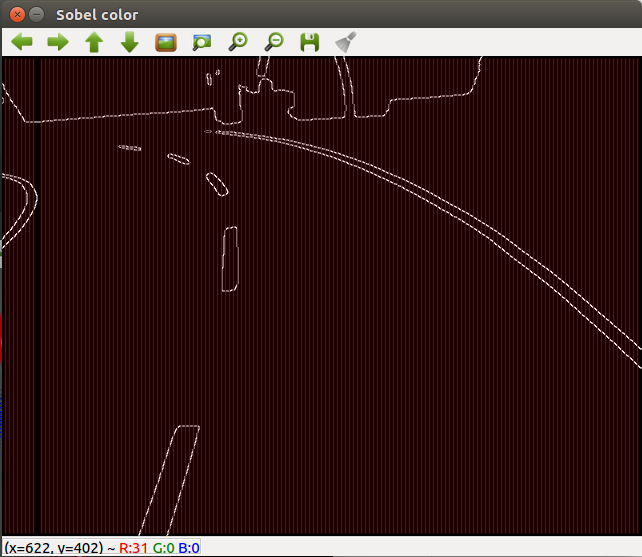
\includegraphics[width=0.45\textwidth]{./Bilder/Case1_withoutCropped.png}\label{fig:Case1_withoutCropped}}
  \hfill
  \subfloat[Standard Hough Transformation with Cropping Image]{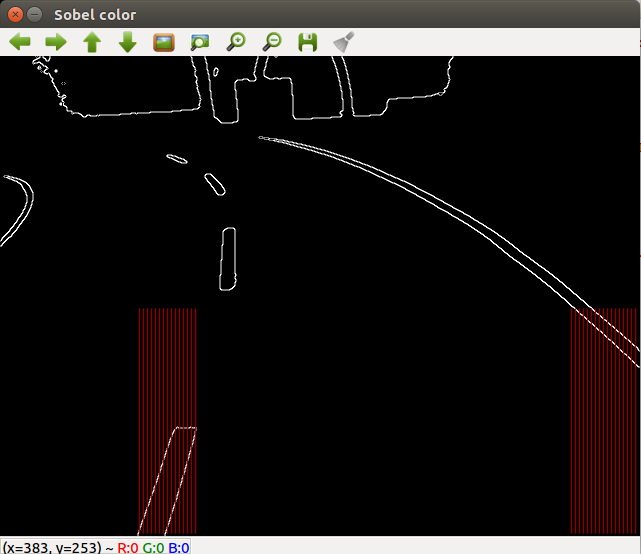
\includegraphics[width=0.45\textwidth]{./Bilder/Case1_withCropped.png}\label{fig:Case1_withCropped}}
  \caption{Detecting Lane Positions}
\end{figure}


As previously explained, the positions of the two lanes (right and middle) were detected. However, even if more than the lower 230 pixels of the frame are used, the positions of the all lanes can be detected (if all three lanes can be seen in the frame), but in this case, another problem occurs. As seen in Figure \ref{fig:Case1_StandardHough_Curve}, the Standard Hough Transformation is implemented for the lower 380 pixels of the frame. As shown in the same Figure, if there is a curve, everything works fine and the positions of the all lanes can be detected. However, if there is a straight lane like in Figure \ref{fig:Case1_StandardHough_geradeaus}, the position of the lanes can not be detected correctly.  The beginning of the middle lane is grouped with the left lane, so it causes lane detection problems. In other words, there are again three different groups for three different lanes but each group of red lines fails to separate the lanes clearly from each other. As a result, the correct starting points of the middle and left lanes are not able to be found. In order for the lanes to be detected clearly, the Standard Hough Line Transformation must be used for only the lower 240 pixels of the frame. At the end of this step, the positions of the middle and right lanes are detected.




\begin{figure}[H]
  \centering
  \subfloat[Standard Hough Transformation in the Curve Lane]{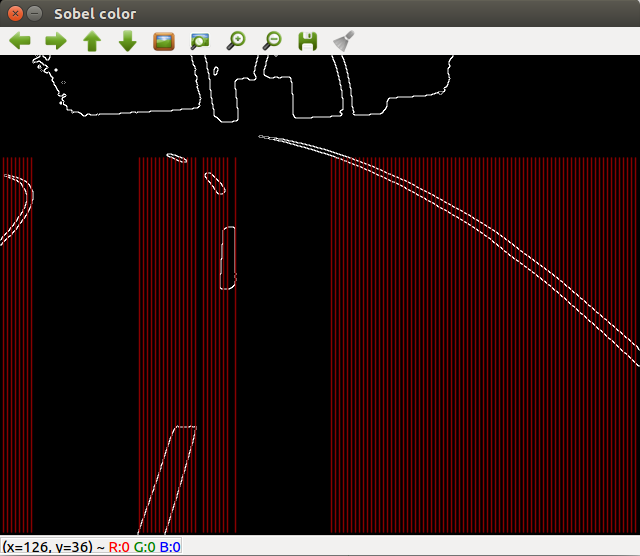
\includegraphics[width=0.45\textwidth]{./Bilder/Case1_StandardHough_Curve.png}\label{fig:Case1_StandardHough_Curve}}
  \hfill
  \subfloat[Standard Hough Transformation in the Straight Lane]{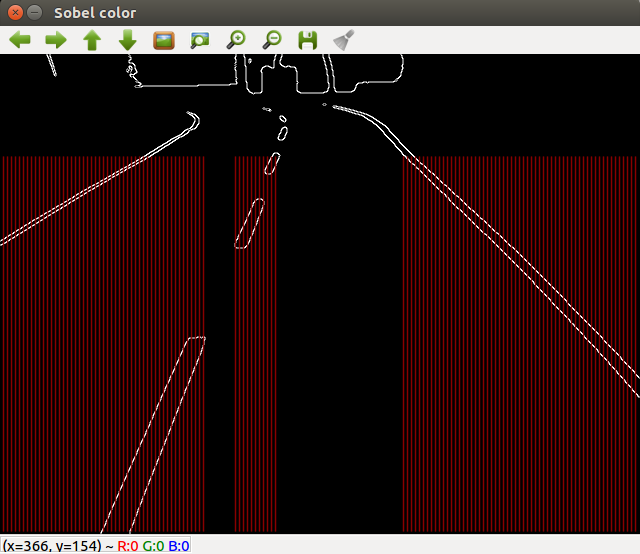
\includegraphics[width=0.45\textwidth]{./Bilder/Case1_StandardHough_geradeaus.png}\label{fig:Case1_StandardHough_geradeaus}}
  \caption{Standard Hough Transformation Detection Problem}
\end{figure} 


{Step 3 : }After the positions of the middle and right lanes are detected, the Probabilistic Hough Transformation must be implemented. Probabilistic Hough Transformation finds the pixels, which are on the edges of the lanes. The Probabilistic Hough
Transformation is a bit different than Standard Hough Line Transformation because Standard Hough Transformation is more suitable for straight lanes. However, if there is a curve, the Standard Hough Transformation is not able to detect lanes very well. As previously mentioned in Section \ref{sec:Standard Hough Line Transformation}, a line can be represented as y = mx+c, or in parametric form, as $\rho$ = x cos $\theta$ + y sin $\theta$, where $\rho$ is the perpendicular distance from origin to the line, and $\theta$ is the angle formed by this perpendicular line and the horizontal axis measured counter-clockwise. However, the process differs in the case of the Probabilistic Hough Transformation. A line is represented by two or more points. If the Probabilistic Hough Transformation finds at least two points from the same line, it represents the two end points of these lines.

In this project, the function for the Probabilistic Hough Transformation from OpenCV is used. It detects lines, but all lanes consist of small lines, even if they are curved. In this project, these small lines on the lanes are detected. These small lines have start and end points, so instead of the drawing these small lines, the start and end points of these small lines are shown. All of these points (pixels) are on the lanes. As previously explained in Section \ref{sec:Probabilistic Hough-Transformation}, the parameters must be set for Probabilistic Hough Transformation. Here, the value '$\rho$' is the resolution in pixels. In this project, this value is set as two and it means that for every two pixels, lines are searched for.  Another value in this function is '$\theta$', which is the resolution in radians. In the Standard Hough Transformation, this value is chosen as 180 degrees, which means only vertical lines can be detected. However, in the Probabilistic Hough Transformation, this value is set as one pixel, which is the minimum value that can be chosen. The 'threshold' value decides the minimum number of points in the same line in order to detect a line. This value used in this project is two because it is enough to detect a line if there are only start and end points in a line. Another parameter in this function is 'minLinLength', which is the minimum length of the line. In this project, Probabilistic Hough Transformation is used to detect small lines in the lanes, so this value must be very small. In this project, two is selected as this value, because if there are two pixels next to each other in the same lane, these pixels must be detected. The last parameter of the Probabilistic Hough Transformation function is 'maxLineGap', which allows for the detection of lines which are farther away from each other than the value selected for this parameter. In order to detect a large number of Hough Points, which is needed for stable line detection, the value selected is two, meaning that the Hough Points farther than two pixels away from each other are detected. All of these parameters can be changed and affect the computing time. 


\begin{figure}[H]
  \centering
  \subfloat[Original Image with Probabilistic Hough Transformation without Cropping]{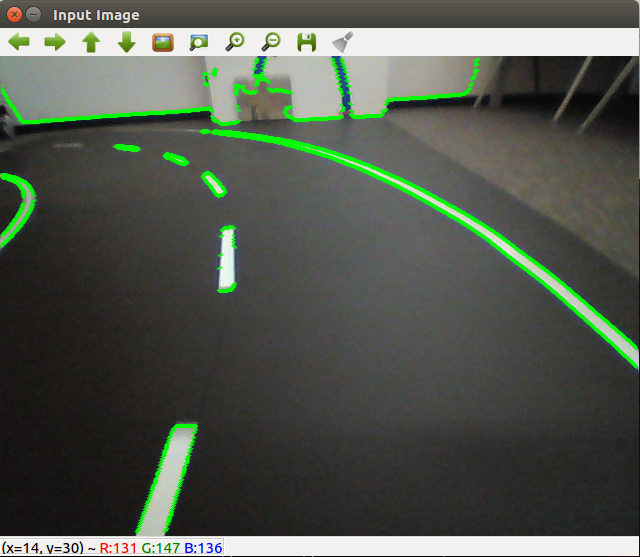
\includegraphics[width=0.45\textwidth]{./Bilder/Case1_HoughPoints_Original.png}\label{fig:Case1_HoughPoints_Original}}
  \hfill
  \subfloat[Original Image with Probabilistic Hough Transformation with Cropping]{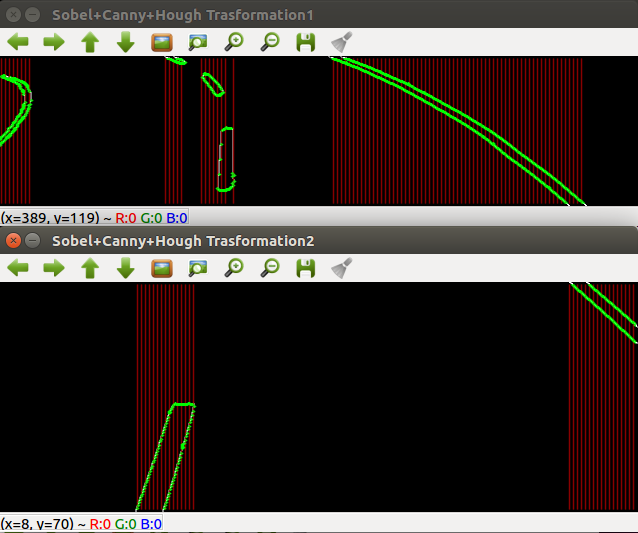
\includegraphics[width=0.45\textwidth]{./Bilder/Case1_HoughPoints_Sobel.png}\label{fig:Case1_HoughPoints_Sobel}}
  \caption{Probabilistic Hough Transformation Points}
\end{figure} 
 
In Figure \ref{fig:Case1_HoughPoints_Original} and Figure \ref{fig:Case1_HoughPoints_Sobel}, the Probabilistic Hough Transformation Points (green pixels) are shown. The Probabilistic Hough Transformation detected a large number of pixels. By changing the parameters of the Probabilistic Hough Transformation found in OpenCV, fewer Hough Points on the lanes are detected, but detecting too few Hough points can also cause some problems for lane detection. On the other hand, detecting a large number of Hough Points results in more computing time, which is undesirable. So in this case, the parameters of Probabilistic Hough Transformation function in OpenCV must be optimized. Thanks to optimization, the best solution (less computing time and good lane detection) is found.  As previously mentioned, detecting a larger number of Hough Points increases the computing time. Due to this reason, the Probabilistic Hough Transformation is not used in the entire frame. As seen in Figure \ref{fig:Case1_HoughPoints_Original}, in the upper pixels of the frame, there are many Probabilistic Hough Points which are not relevant to the lane, so the upper 100 pixels of the frame are cropped before the Probabilistic Hough Transformation is implemented. In Figure \ref{fig:Case1_HoughPoints_Sobel}, the Probabilistic Hough Points are just on the lines. When the upper 100 pixels are cropped, the algorithm is much faster when compared to leaving using the entire frame.

\textbf{Step 4 : }It is now known in which pixel columns the middle and right lanes lie (Step 2), and the points (pixels) on the lanes are also shown thanks to Probabilistic Hough Transformation (Step 3), and after these two steps, the starting points (pixels) of the lanes can be found. In order to do that, the Hough Points for each group of Hough lines found in Step 2 are compared with each other, and then the lowest pixels in the columns should be found. If the camera can see three lanes, then the different starting points for the three different lanes must be found. This means that this process must be done for all lanes which can be seen in the frame. As seen in Step 2, the position of the left lane is not detected, although the camera is able to see the left lane. Because the left lane is not seen in the lower 230 pixels, the position of the left lane is not detected. In this case, the Hough Points, which lie to the left of the middle lane, are compared with each other and then the lower pixel is found. It is the starting point (pixel) of the left lane.


\textbf{Step 5 : }The next step in this method is getting the Hough Points which are relevant to the lanes. Now, for each lane, the Hough Points must also be grouped. In order to get the Hough Points relevant to the lanes,  the 'rectangle method' is used. In the ectangle method, a rectangle is drawn for each lane at the starting point found in Step 4, and the coordinates of all of the Hough Points in that rectangle are saved in a vector. The highest Hough Points in the rectangle must then be found. From that point, another rectangle must be drawn, but the sizes of the rectangles become progressively smaller, because the objects seem smaller the further away they are from the camera. The sizes of the rectangles are also similar for left and right lanes, but there is an exception with regard to the middle lane. The middle lane has dashed lines, so the rectangles in the middle lane must be bigger than in the left and right lanes. As seen in Figure \ref{fig:Case1_Rectangles} (rectangles shown in blue), with this method, the noise and the Hough Points not relevant to the lanes are removed. For the 'rectangle method', a function is defined in the source code. The inputs of this function are: the input image, in which also the Probabilistic Hough Transformation was used; the starting point of the lane; the vector of the Hough Points; and the lane for which this function is used must also be defined. In which lane the rectangles are to be drawn must also be known, because as previously mentioned, due to the dashed lines in the middle lane, the size of the rectangles in the middle lane is bigger when compared to the rectangles in the left and right lanes.


\begin{figure}[H]
 \centering
  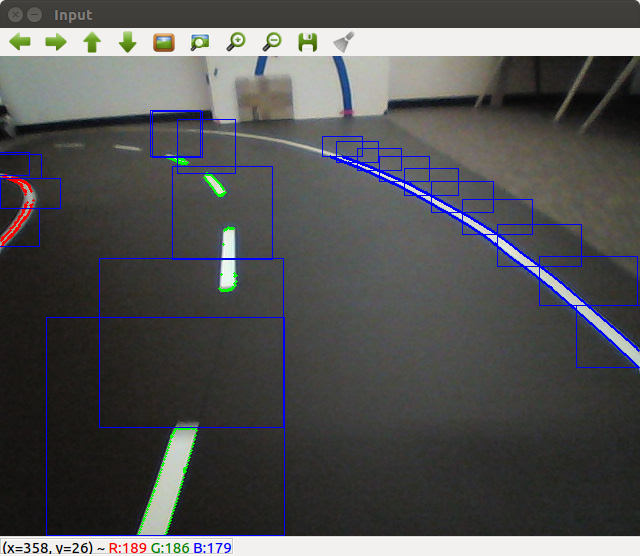
\includegraphics[width=0.45\textwidth]{./Bilder/Case1_Rectangles.png}
	\caption{Rectangle Method}
	\label{fig:Case1_Rectangles}
\end{figure}


\textbf{Step 6 : }The next step of this method is curve fitting. Curve Fitting is an algorithm which gives a mathematical description and this mathematical description provides the best fit for a series of data points. But in this master's thesis, the curve fitting to be performed is modified. In this curve fitting, the coordinates of Hough Points are used but the x and y coordinates of these Hough Points are swapped, because the y-axes of these coordinates have more range than the x-axes. As a result, this swap raises the stability of the curve fitting.

After using the Hough Points as input, three different mathematical equations are produced. One of these equations is for the left lane, another is for the middle lane, and the last equation is for the right lane. In order to produce these equations, naturally, only the relevant Hough points are used. For example, for left lane curve equation, only the Hough Points from the left lane are used. For  the curve fitting, a function is implemented in the source code. One of the inputs is the input image. Another input of the function is the vector of the Hough points which are relevant for that lane. In other words, if the curve fitting function is used for the right lane, then the Hough points relevant to right lane must be used. These points are grouped in Step 5 with the rectangle method.  If  it is desired for the fitted curves to be shown in the frame, in order to differentiate the fitted curves from each other, colors can be chosen. As a result, the color value is also another input in this function. Available colors of fitted curves are red, green, and blue. Other colors can also be used. The last input value of this function is 'IPM'. In order to track the lanes, the equations of the fitted curves must be given from the bird's-eye perspective so the Inverse Perspective Mapping (IPM) algorithm must be applied. For IPM, a function from OpenCV, which is called 'findHomography', was used. Thanks to this function, all Probabilistic Hough Points on the lanes can be converted to the bird's-eye perspective. It is also possible to convert all pixels from the camera perspective to bird's-eye perspective, but in that case, it is also necessary to convert 640x480 pixels, which means 307200 pixels in total. Because this is computationally expensive, only the Hough Points relevant to the lanes are converted. Much fewer pixels are converted when compared to converting all pixels in the frame. The IPM algorithm is very computationally expensive in and of itself, so converting fewer pixels makes this method more efficient. As a result, the inputs of the fitted curves are the transformed Hough Points, which are converted from the camera perspective to the bird's-eye perspective.The output equations of the fitted curves are therefore also for the bird's-eye view.
 
\textbf{Step 7 : }The next step of this method is plotting the fitted curves produced by the curve fitting function. In this case, the fitted curve starts from the first pixel and continues to the 480th pixel vertically and the output values of the equation for each pixel in the column are found. For each line, the fitted curves are plotted in different colors. To be sure if the lanes are correctly detected, the input image is also transformed and the fitted curves are plotted in Figure \ref{fig:Case1_CurveFitting}.

		 	
\begin{figure}[H]
  \centering
  \subfloat{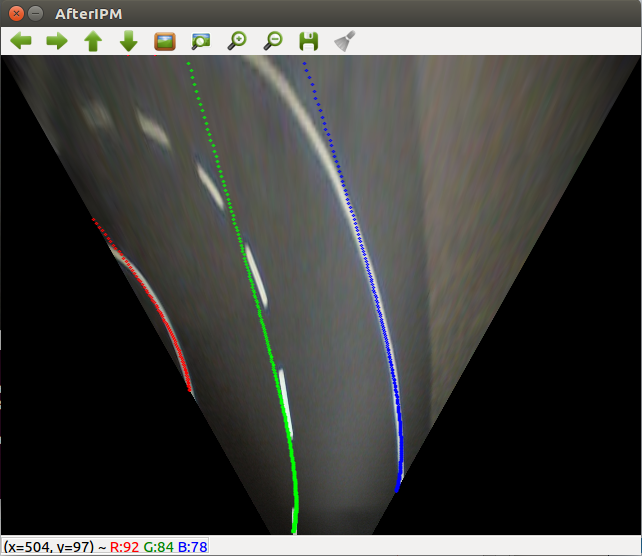
\includegraphics[width=0.45\textwidth]{./Bilder/Case1_CurveFitting.png}\label{fig:Case1_CurveFitting}}
  \caption{Curve Fitting}
\end{figure} 


\textbf{Step 8 : }The last step of this method is publishing the coefficients of the equations of the fitted curves from the bird's-eye view. In order to activate the automobile for autonomous driving, only the equations of the fitted curves are needed. For this step, a ROS Topic must be created. The frequency of the rostopics can be adjusted.

%



\subsection{Method 1(b) : Resize + Hough Transformation + Rectangle Method + Curve Fitting + IPM}\label{sec:Case 4}


This method is very similar to Method 1 in Section \ref{sec:Case 1}. The only difference between these two methods is that in the Method 1, the resolution of the frame is 640x480 pixels and in this method, the resolution of the frame is four times smaller, with a resolution of 320x240 pixels. In order to reduce the resolution of the frame, the width and height values in pixels must be sent to the camera before it is started. While reducing the resolution of the frame has some advantages, it also has some disadvantages. These will be explained in the Chapter \ref{cha:Evaluation and Discussion}. The output frame of this method is shown in Figure \ref{fig:Case4_OutputImage}.


\begin{figure}[H]
  \centering
  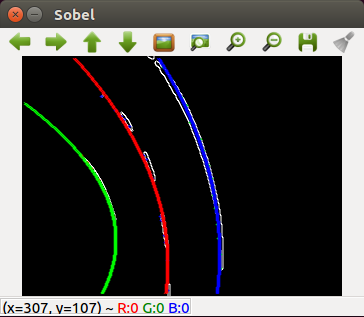
\includegraphics[width=0.45\textwidth]{./Bilder/Case4_OutputImage.png}
  \caption{Output Image(320x240 pixels resolution)}
  \label{fig:Case4_OutputImage}
\end{figure}






\subsection{Method 2 : IPM + Hough Transformation + KNN + Curve Fitting}\label{sec:Case 2}

\begin{figure}[H]
 \centering
  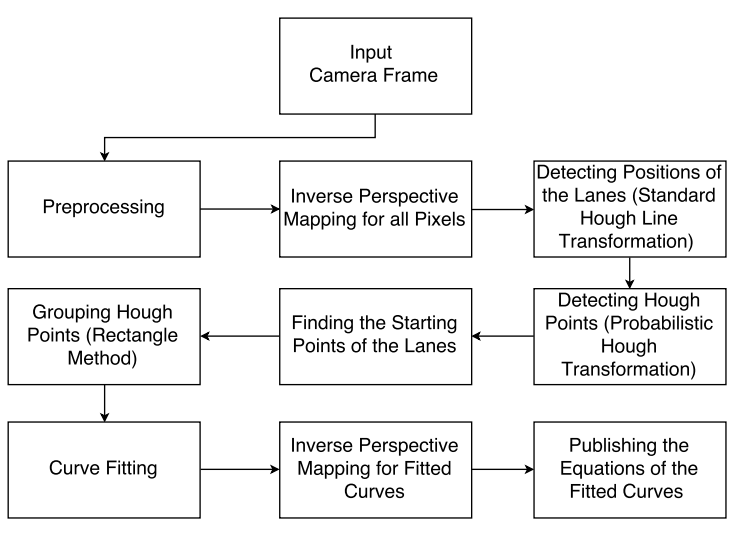
\includegraphics[width=1\textwidth]{./Bilder/Case2_BlockDiagram.png}
	\caption{Block Diagram of Method 2}
	\label{fig:Case2_BlockDiagram}
\end{figure}

\textbf{Step 1 : }As previously mentioned, the preprocessing part is common for all methods. So in this method, the preprocessing part was also the first step.

\textbf{Step 2 : }In this method, the frames are taken by the camera, then the upper 100 pixels of the frame are cropped, otherwise, the lanes appear far away from the bird's-eye perspective and thus appear smaller (more info in the Section \ref{sec:Inverse Perspective Mapping}). Then the cropped frames are converted from the camera perspective to the bird's-eye view perspective. In Section \ref{sec:Case 1} (Method 1), only the curve fitting pixels were converted from the camera perspective to the top of the track perspective. The time needed to convert 640x380 pixels (243200 pixels in total) is a bit more when compared to Method 1. The original frame, which can be seen in Figure \ref{fig:Case2_InputImg}, is converted to the frame which can be seen in Figure \ref{fig:Case2_IPM} by OpenCV 'findHomography' function.

 
\begin{figure}[H]
  \centering
  \subfloat[Original Image]{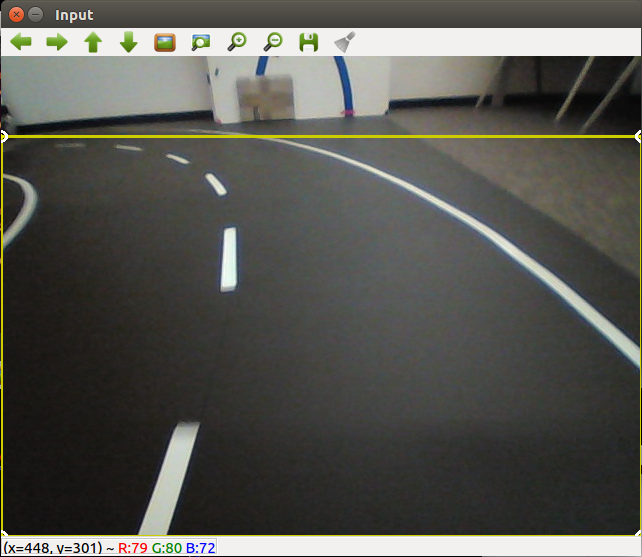
\includegraphics[width=0.45\textwidth]{./Bilder/Case2_InputImg.png}\label{fig:Case2_InputImg}}
  \hfill
  \subfloat[A Image with Inverse Perspective Mapping]{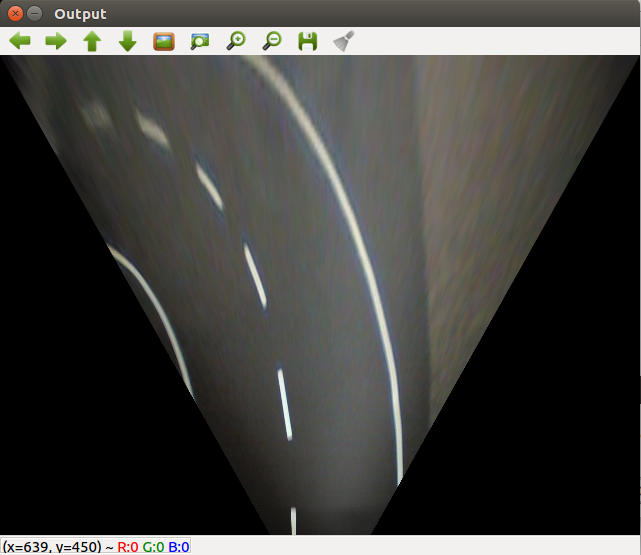
\includegraphics[width=0.45\textwidth]{./Bilder/Case2_IPM.png}\label{fig:Case2_IPM}}
  \caption{Inverse Perspective Mapping}
\end{figure} 


\textbf{Step 3 : }In Method 1, the Standard Hough Transformation is applied to only the lower 230 pixels. In this methood, it sufficient to apply the Standard Hough Line Transformation to only the last 200 pixels of the frame, because these 200 pixels are able to cover all lanes in the frame. In Figure \ref{fig:Case2_Standard_Hough_Transformation}, all lanes can be distinguished thanks to the Hough lines. 


\begin{figure}[H]
  \centering
  \subfloat{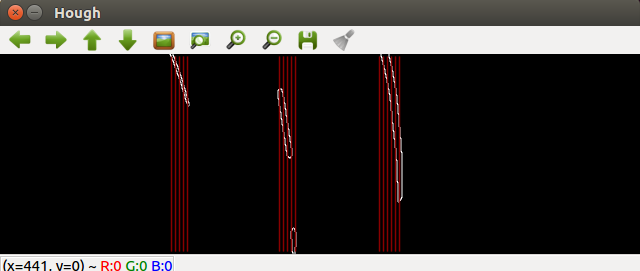
\includegraphics[width=0.45\textwidth]{./Bilder/Case2_Standard_Hough_Transformation.png}\label{fig:Case2_Standard_Hough_Transformation}}
  \caption{Standard Hough Line Transformation after IPM Method}
\end{figure} 



\textbf{Step 4 : }After finding which pixel columns the lanes lie between in Step 3, the Probabilistic Hough Transformation was used. Thanks to Probabilistic Hough Transformation, the Hough Points appear on the lanes. As mentioned in Method 1 in Section \ref{sec:Case 1}, there are some parameters in Probabilistic Hough Transformations, so the number of Hough Points can be descreased or increased. Decreasing the number of Hough Points also decreases the computing time but decreasing the number of Hough Points by too much can decrease the accuracy of lane detection. Therefore, the parameters must be set in an optimal way.

\textbf{Step 5 : }We have already found out which pixel columns the lanes lie between. The Hough Points must now be grouped according to lanes. If the camera can see all three lanes, then there must also be three different groups of Hough Points. However, if there is a curve, the camera can see just the right and middle lane, so the Hough Points must be grouped into two groups in this case. For each lane, the starting points of the lanes must be found. For that, all Hough Points in a group must be compared with each other. The Hough Points which are the closest to the bottom of the frame are the starting points.

\emph{\color{green}\textbf{Step 6 : }The next step of this method is the k-nearest neighbors algorithm (KNN). KNN is a learning algorithm. Here KNN is used instead of the rectangle method used in Method 1. The KNN algorithm divides the frames into some equal-sized pieces. The nearest neighbor points are found in each piece. This process begins from the starting points of the lanes which were found in Step 5. The KNN functions are used from OpenCV. There are some parameters in these functions. For example, we can set the number of neighbor points to be found. The parameters must be set optimally, meaning the project must work fast and efficiently.}

\textbf{Step 7 : }After finding the points from KNN in Step 6, which are to be used as the input values of the curve fitting function, then the function of the curve fitting is applied. The advantage of the KNN algorithm is that it does not return so many Hough Points, which are the input values of the curve fitting, when compared to rectangle method. So here, the curve fitting function produces the mathematical equations of the lane much faster when compared to Method 1.

\textbf{Step 8 : }After the equations of the fitted curves for each of the lanes are calculated, these equations have to be plotted like in Method 1. Here, the x and y coordinates of the Hough Points were also swapped in order to get more stable curves. For each of the vertical pixels, the results of all of the equations were plotted in the frame.


\textbf{Step 9 : }The last step of this method is also to publish the coefficients of the equations of the fitted curves of each of the lanes which can be seen by the camera.


\begin{figure}[H]
  \centering
  \subfloat{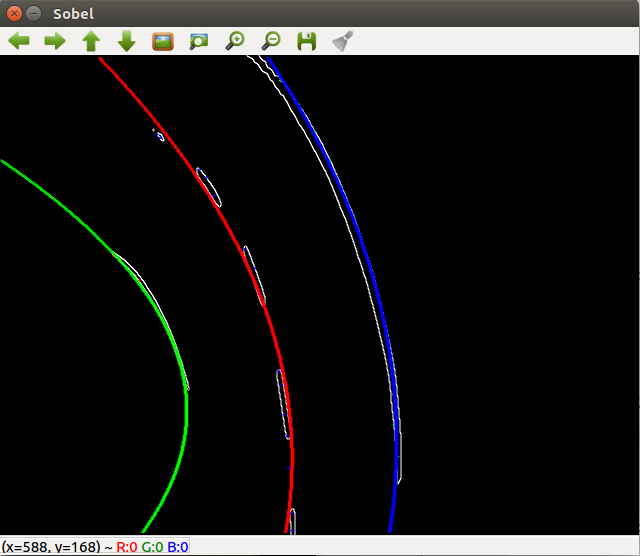
\includegraphics[width=0.45\textwidth]{./Bilder/Case2_OutputImage.png}\label{fig:Case2_OutputImage}}
  \caption{Output Image}
\end{figure} 



\subsection{Method 2(b) : Resize + IPM + Hough Transformation + KNN + Curve Fitting}\label{sec:Case 5}

This method is very similar to Method 2, which was described in Section \ref{sec:Case 2}. In the Method 2, the resolution of the frame is 640x480 pixels and in this method, the resolution of the frame is 320x240 pixels. In Chapter \ref{cha:Evaluation and Discussion}, the effects of the reducing the resolution of the frame will be described. The output frame of this method is shown in Figure \ref{fig:Case5_OutputImage}.


\begin{figure}[H]
  \centering
  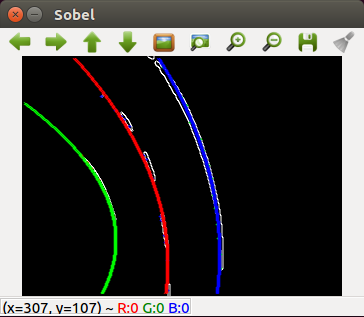
\includegraphics[width=0.45\textwidth]{./Bilder/Case5_OutputImage.png}
  \caption{Output Image(320x240 pixels resolution)}
  \label{fig:Case5_OutputImage}
\end{figure}




\subsection{Method 3 : IPM + Hough Transformation + Rectangle Method + Curve Fitting}\label{sec:Case 3}

This method is a composite method of the Method 1 in Section \ref{sec:Case 1} and Method 2 in Section \ref{sec:Case 2}. As in Method 2, at the beginning of this method, the preprocessing part is applied, and then Inverse Perspective Mapping for all pixels is implemented. After that, for 200x640 pixels, the Standard Hough Transformation is used and then for all pixels Probabilistic Hough Transformation is implemented. Until this point, the implementation is completely identical to Method 2. In Method 2, however, at the point in the process where the k-nearest neighbours (KNN) method is used, the rectangle method used in Method 1 in Section \ref{sec:Case 1} is applied. There is, however, a difference between the rectangle method utilized here and the rectangle method from Method 1. In Method 1, the size of rectangles decreased progressively. However, in this method, the size of the rectangles is always the same because the Inverse Perspective Method(IPM) is used at the beginning. As a result, the lanes are shown from the top of track. The size of the rectangles in the middle lane is bigger than the size of the rectangles in the left and right lanes, however. Because of the dashed lines, it was necessary to use larger rectangles in the middle lane.

After the rectangle method is used, the curve fitting method is used. As with the other methods, the x and y coordinates of Probabilistic Hough Points are swapped after the rectangle method is applied. Thanks to this swap, the curve fitting is more accurate. After producing three different equations for three different lanes, the output values for all pixel columns are calculated and plotted in the frame. In Figure \ref{fig:Case3_OutputImage}, the fitted curves are shown.

The last step of this method is as in the others: to publish the equations of the fitted curves produced from the lanes. These fitted curves are published with Ros Topics.

\begin{figure}[H]
 \centering
  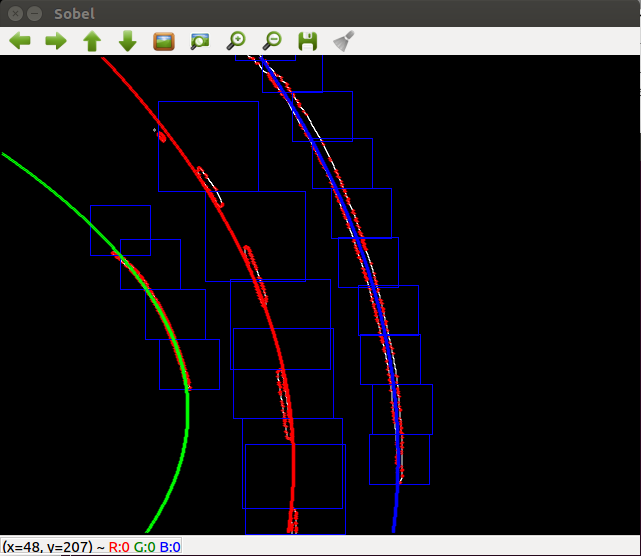
\includegraphics[width=0.45\textwidth]{./Bilder/Case3_OutputImage.png}
	\caption{Output Image}
	\label{fig:Case3_OutputImage}
\end{figure}











%


